\documentclass{beamer}
\usepackage[utf8]{inputenc}
\usepackage[T1]{fontenc}
\usepackage[english,main=french]{babel}
\usepackage[babel=true]{csquotes}
\usepackage{graphicx}
\usepackage[export]{adjustbox}
\usepackage{amsmath}
\usepackage{algorithm2e}
\usepackage{hyperref}
\usepackage{listings}
\usepackage[toc,page]{appendix}


\graphicspath{ {../images/} }
\usetheme{Copenhagen}
\setbeamertemplate{page number in head/foot}[totalframenumber]
\setcounter{tocdepth}{2}
\lstset{
    basicstyle=\ttfamily,
    breaklines=true,
    showstringspaces=false,
    keywordstyle=\color{blue},
    commentstyle=\color{red}
}


\title{Soutenance de stage de 2\ieme année}
\subtitle{Speeding up LHCb software through compilation optimization}
\author{Oscar Buon}
\date{4 septembre 2023}


\begin{document}

\begin{frame}
    \centering
    \begin{minipage}{0.2\textwidth}
        
\includegraphics[width=\textwidth]{logo_ISIMA_INP.png}
    \end{minipage}\hfill
    \begin{minipage}{0.2\textwidth}
        
\includegraphics[width=\textwidth]{logo_CERN.png}
    \end{minipage}\hfill
    \begin{minipage}{0.2\textwidth}
        
\includegraphics[width=\textwidth]{logo_LHCb.png}
    \end{minipage}

    \maketitle

    Jury: Sébastien Ponce, Mamadou Kanté, Claude Mazel
\end{frame}


\part{Introduction}
\section*{Introduction}

\begin{frame}
    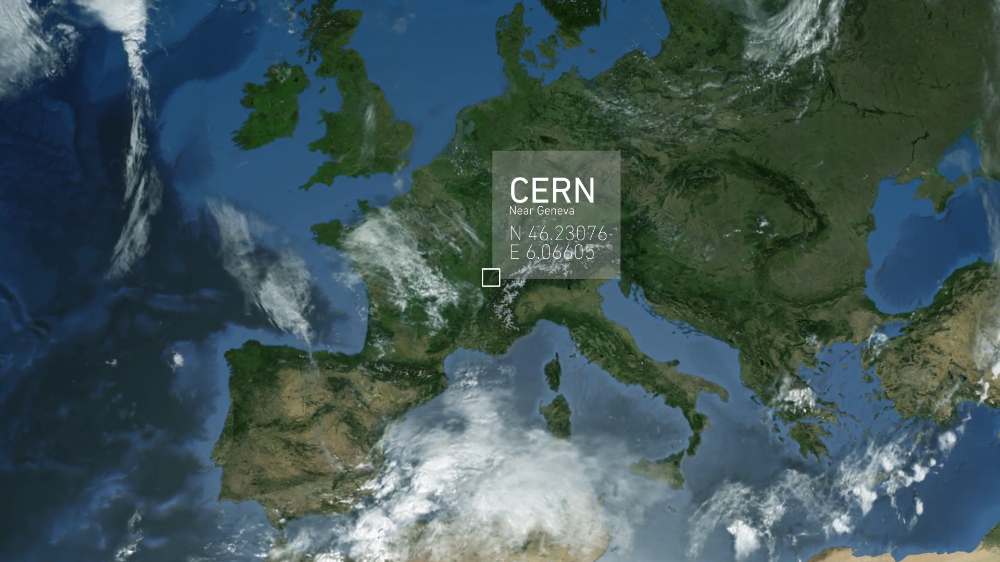
\includegraphics[width=\textwidth]{video/Geneva.png}
\end{frame}

\begin{frame}
    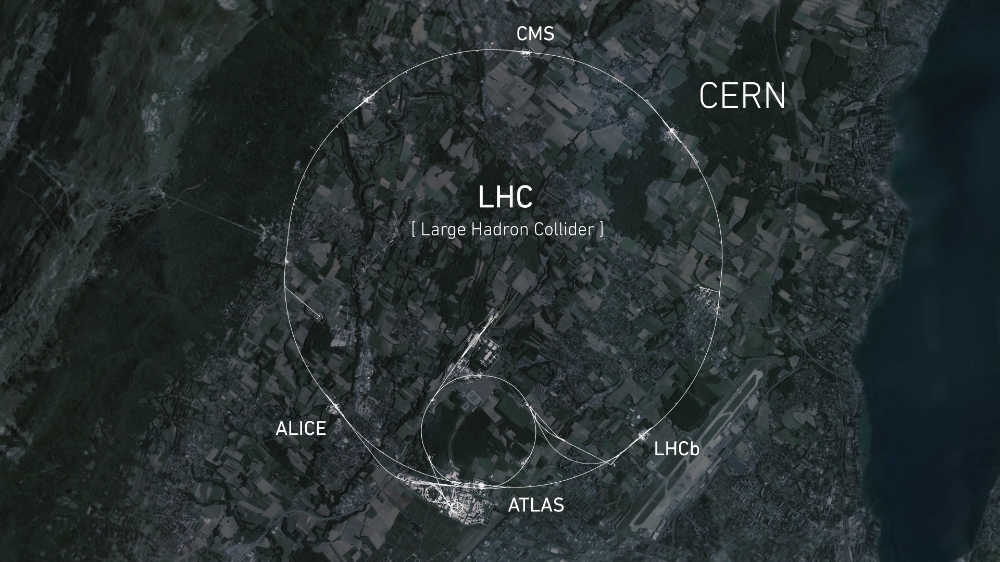
\includegraphics[width=\textwidth]{video/map.png}
\end{frame}

\begin{frame}
    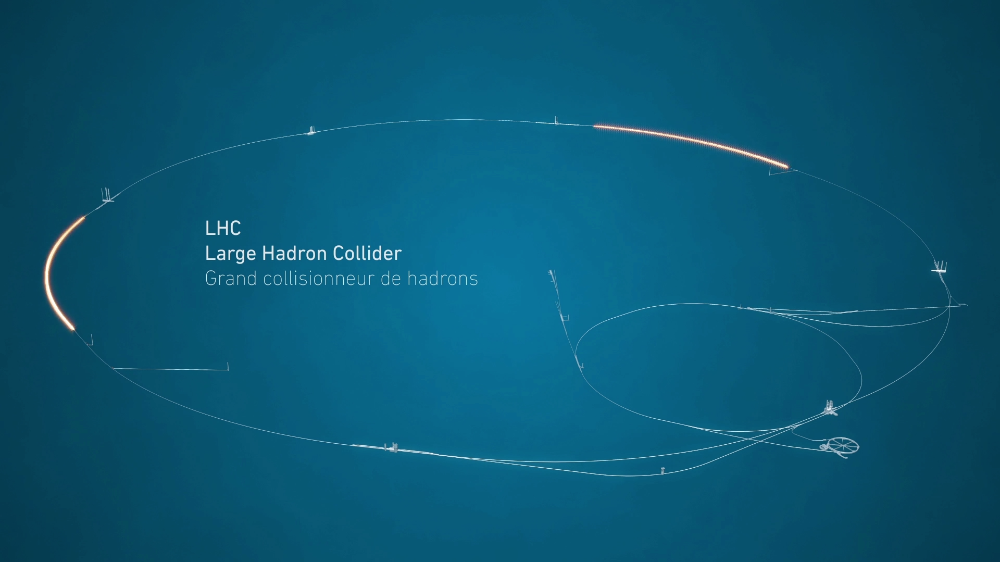
\includegraphics[width=\textwidth]{video/lhc.png}
\end{frame}

\begin{frame}
    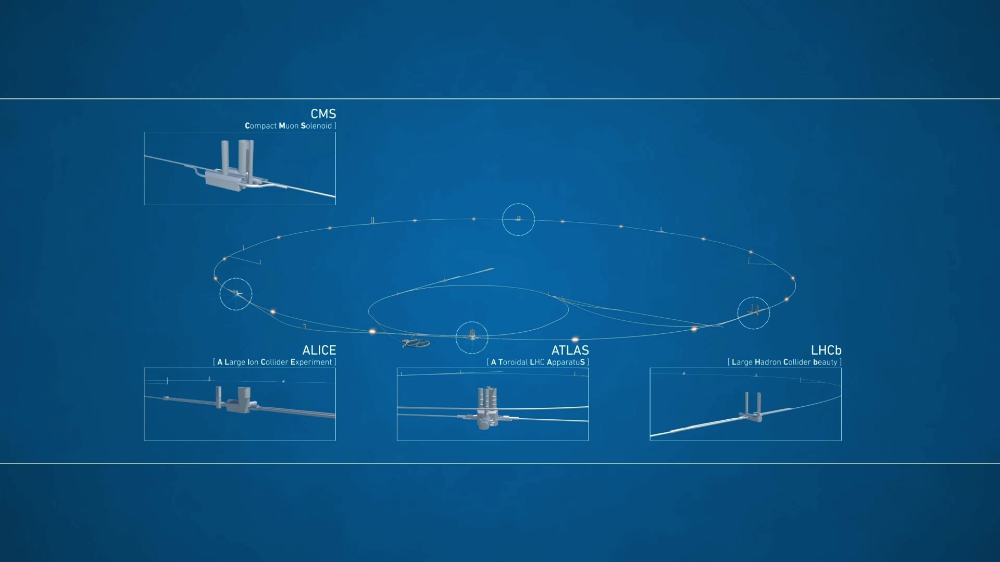
\includegraphics[width=\textwidth]{video/detectors.png}
\end{frame}

\begin{frame}
    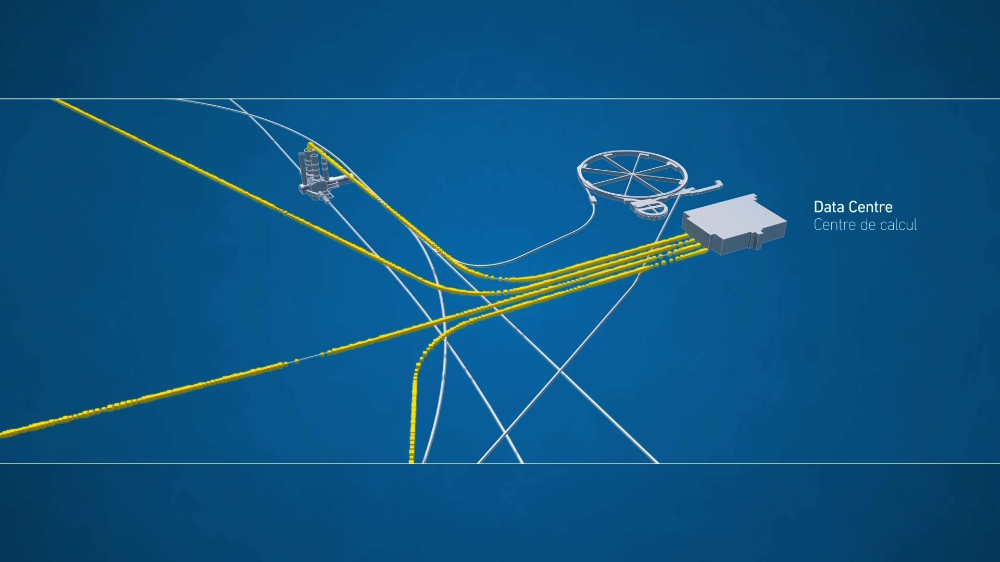
\includegraphics[width=\textwidth]{video/data_center.png}
\end{frame}

\begin{frame}
    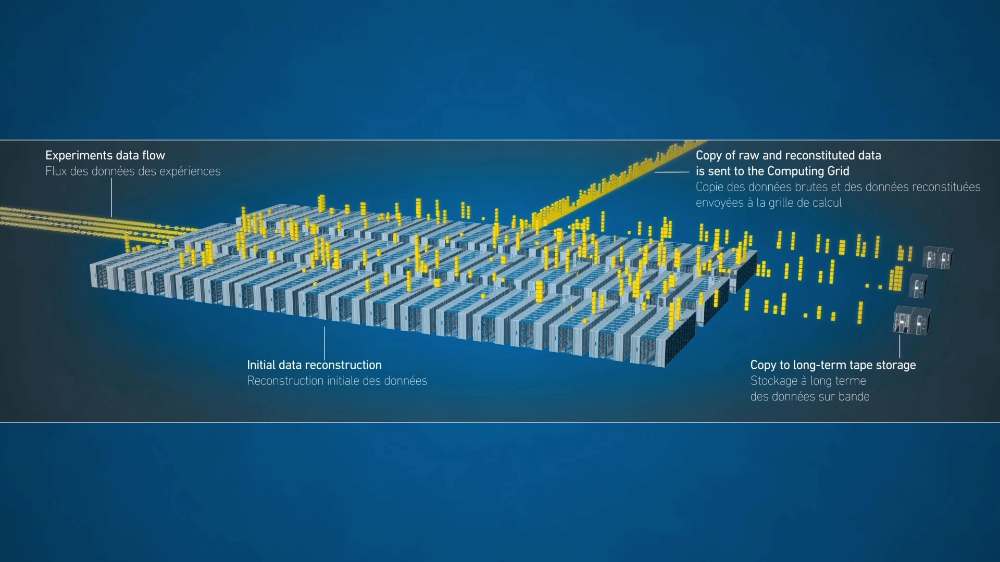
\includegraphics[width=\textwidth]{video/processing.png}
\end{frame}

\begin{frame}
    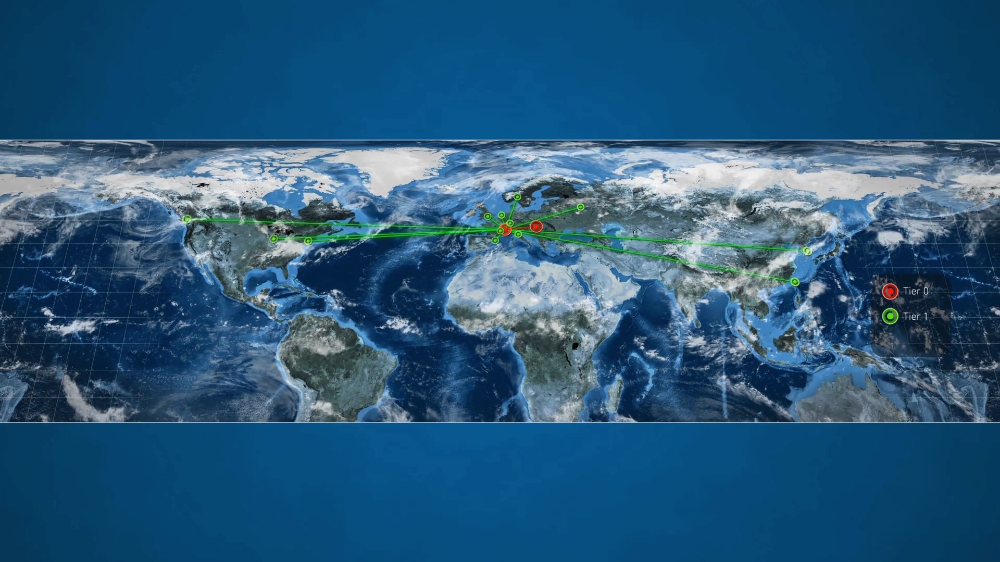
\includegraphics[width=\textwidth]{video/grid.png}
\end{frame}

\begin{frame}
    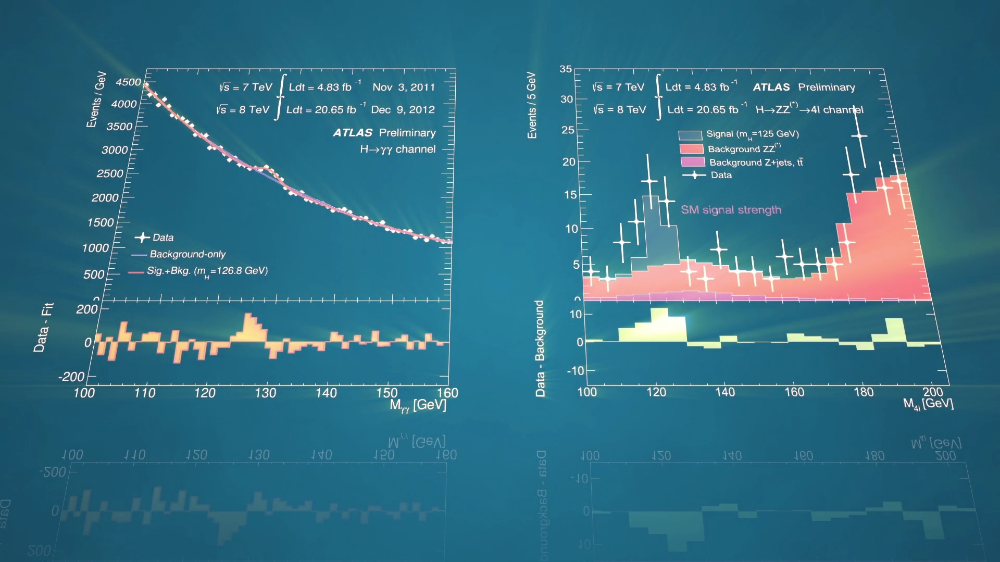
\includegraphics[width=\textwidth]{video/graphs.png}
\end{frame}

\begin{frame}
    \frametitle{LHCb}

    \centering
    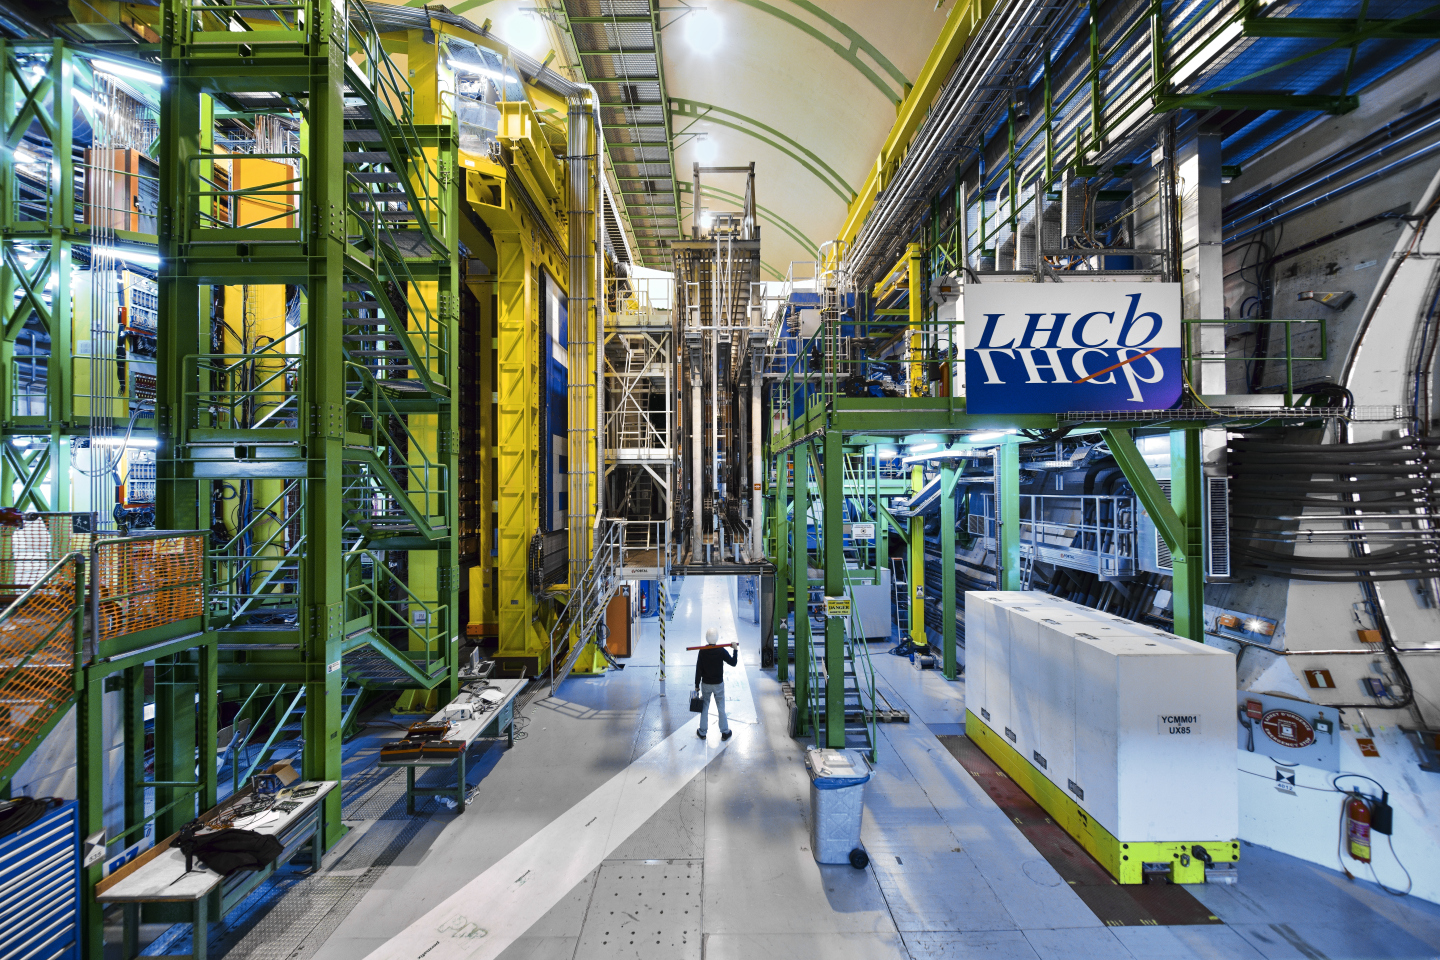
\includegraphics[width=0.9\textwidth]{LHCb.jpg}
\end{frame}

\begin{frame}
    \frametitle{Computing group}

    \begin{itemize}
        \item Gère l'infrastructure logicielle de LHCb ;
        \item Maintient les programmes de traitement des données issues du détecteur.
    \end{itemize}

    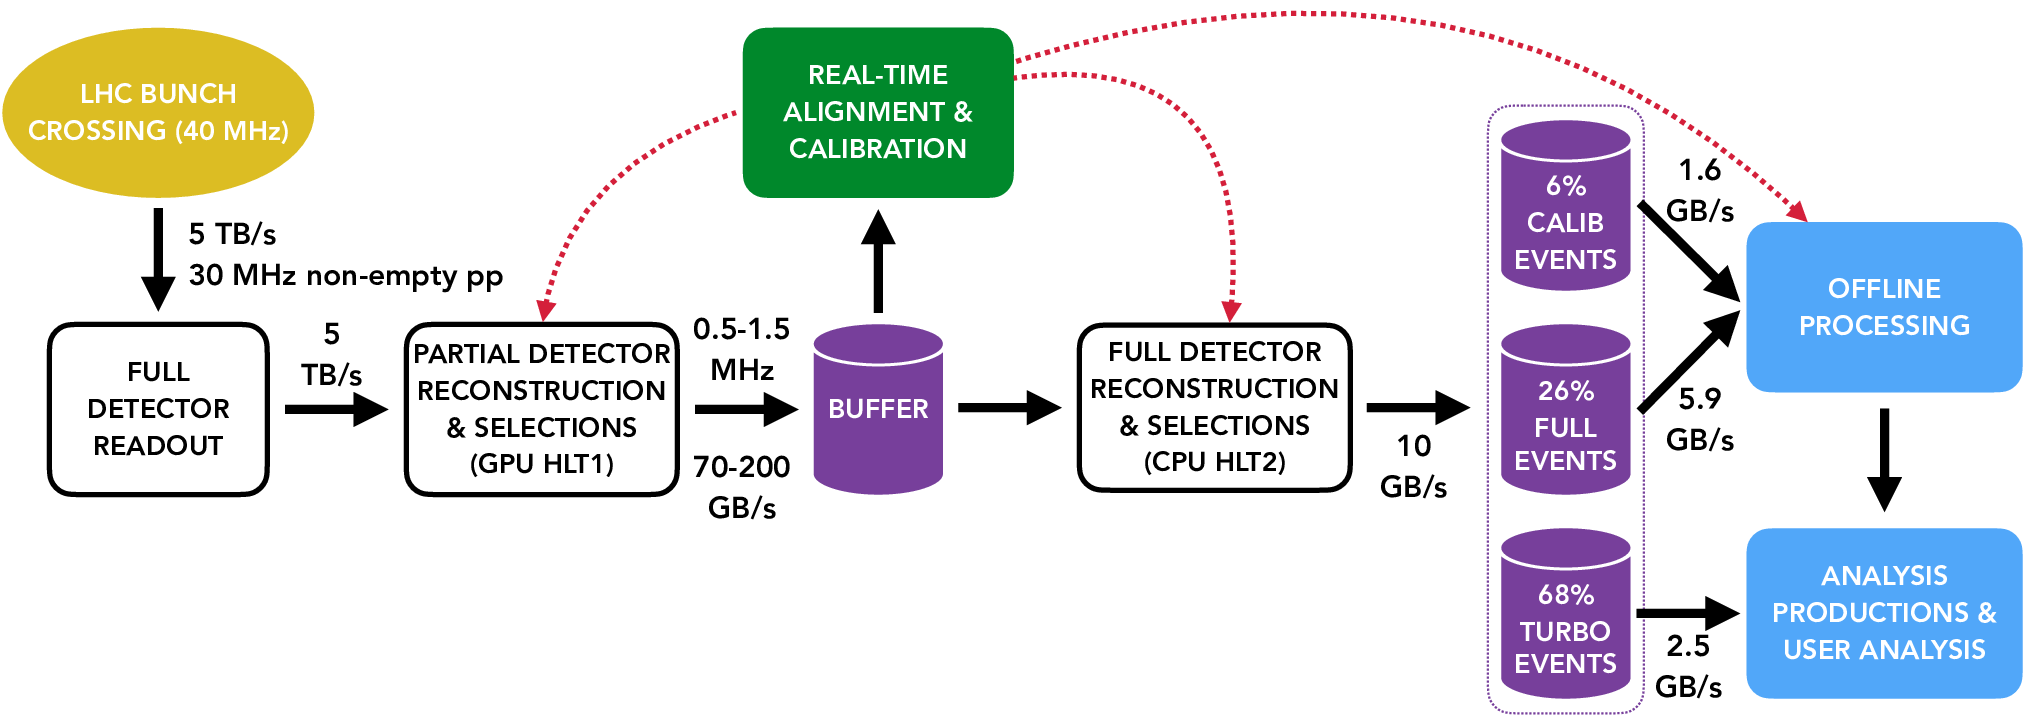
\includegraphics[width=\textwidth]{LHCb_stack.png}
\end{frame}

\begin{frame}
    \frametitle{Pile LHCb}

    \begin{itemize}
        \item Root
        \item Gaudi
        \item LHCb
        \item Lbcom
        \item Rec
        \item Allen
        \item Moore
        \item ...
    \end{itemize}
\end{frame}

\begin{frame}
    \frametitle{Pile LHCb}

    \begin{itemize}
        \item Centaines de contributeurs ;
        \item Millions de lignes de codes
        \item dont certaines ont plus de 20 ans.
    \end{itemize}
\end{frame}

\begin{frame}
    \frametitle{Objectif du stage}

    \begin{itemize}
        \item Le traitement a un coût important ;
        \item Besoin d'accélérer / optimiser les calculs ;
        \item Plusieurs méthodes étudiées.
    \end{itemize}
\end{frame}


\part{Body}
\begin{frame}
    \tableofcontents
\end{frame}

\section{Bibliothèques et modules statiques}

\begin{frame}
    \tableofcontents[currentsection]
\end{frame}

\begin{frame}[fragile]
    \frametitle{Structure du software}

    \begin{itemize}
        \item Programmes découpés en morceaux ;
        \item Facilité de développement \& raisons historiques ;
        \item Plusieurs centaines de bibliothèques.
    \end{itemize}
\end{frame}

\subsection{Types de bibliothèques}

\begin{frame}[fragile]
    \frametitle{Types de bibliothèques}

    \begin{itemize}
        \item STATIC: archive de fichiers objets qui sont fusionnés à l'exécutable au moment du link.
        \item SHARED: fichier \verb'.so' (Linux) qui est automatiquement linké à l'exécutable au démarrage du programme.
              Permet à plusieurs exécutables d'être linké à une même bibliothèque installée sur le système.
        \item MODULE: pareil qu'une bibliothèque partagée à la différence qu'un module est chargé sur demande via la fonction \verb'dlopen'.
    \end{itemize}
\end{frame}

\subsection{Bibliothèques statiques}

\begin{frame}[fragile]
    \frametitle{Bibliothèques statiques dans Gaudi}

    \begin{itemize}
        \item Gaudi utilise CMake pour compiler.
        \item Nouvelle fonction CMake dans Gaudi pour créer les bibliothèques statiques :
              \begin{itemize}
                  \item Adaptée de celle pour les bibliothèques partagées.
                  \item \verb'gaudi_add_library' $\Rightarrow$ \verb'gaudi_add_static_library'.
                  \item Remplacer \verb'SHARED' par \verb'STATIC' dans l'appel de la fonction CMake \verb'add_library'.
              \end{itemize}
    \end{itemize}
\end{frame}

\subsection{Modules statiques}

\begin{frame}[fragile]
    \frametitle{Static modules}

    Il faut en plus linker avec :
    \begin{itemize}
        \item \verb'-Wl,--whole-archive'
              \begin{itemize}
                  \item sans quoi le linker enlève ce qui semble être du code inutile.
              \end{itemize}
        \item \verb'-Wl,--allow-multiple-definition'
              \begin{itemize}
                  \item car \verb'-Wl,--whole-archive' fait que des symboles sont inclus plusieurs fois.
              \end{itemize}
        \item \verb'-Wl,--export-dynamic'
              \begin{itemize}
                  \item permet aux foncteurs d'accéder aux symboles.
              \end{itemize}
    \end{itemize}

    Ces options ne sont pas recommandées.
    Il peut encore y avoir des bugs, notamment avec les foncteurs.
\end{frame}

\begin{frame}[fragile]
    \frametitle{Gain de performance}

    \begin{center}
        \begin{tabular}{ c c c }
            Optimisation & Amélioration & Intervalle de confiance ($2\sigma$) \\
            Static       & $0.87\%$     & $\pm 0.60\%$
        \end{tabular}
    \end{center}

    \begin{itemize}
        \item Gains non significatifs.
        \item L'exécutable final passe de $ \sim 20 kB $ à $ 2.5 GB $ (\verb'opt+g').
    \end{itemize}
\end{frame}

\section{Profile-guided optimization}

\begin{frame}
    \tableofcontents[currentsection]
\end{frame}

\subsection{Profile-guided optimization}

\begin{frame}
    \frametitle{Profile-guided optimization}

    Le compilateur utilise des heuristiques pour optimiser certains éléments :
    \begin{itemize}
        \item Inlining,
        \item Ordonnancement des blocs,
        \item Allocation des registres,
        \item Spéculation sur les appels virtuels,
        \item Séparation du code mort.
    \end{itemize}
    Ces optimisations peuvent multiplier la rapidité d'exécution.
    Mais certains heuristiques peuvent être faux.
\end{frame}

\begin{frame}
    Une meilleure manière pour le compilateur serait de connaître le comportement à l'exécution.
    Principe du PGO :
    \begin{itemize}
        \item Compiler le programme avec instrumentation ;
        \item Le faire tourner pour créer des profiles (compteurs) ;
        \item Recompiler le programme avec les profiles.
    \end{itemize}
\end{frame}

\subsection{Link-time optimization}

\begin{frame}
    \frametitle{Link-time optimization}

    \begin{itemize}
        \item Un programme C/C++ est composé de translation units.
              \begin{itemize}
                  \item 1 translation unit $ \approx $ 1 fichier .c/.cpp.
              \end{itemize}
        \item Par défaut, le compilateur ne peux pas optimiser à travers plusieurs translation unit.
        \item Le LTO permet au linker d'effecteur des optimisations qui prennent en compte l'ensemble des translation units.
    \end{itemize}
\end{frame}

\subsection{Étapes de compilation finales}

\begin{frame}[fragile]
    \frametitle{Étapes de compilation finales}

    \begin{itemize}
        \item Compiler avec \verb'-fprofile-generate' ;
        \item Faire tourner le programme sur des données représentatives ;
        \item Recompiler le programme avec \verb'-flto -fprofile-use -fprofile-correction'.
    \end{itemize}
\end{frame}

\begin{frame}[fragile]
    \frametitle{Gain de performance}

    \begin{center}
        \begin{tabular}{ c c c }
            Optimisation      & Amélioration & Intervalle de confiance ($2\sigma$) \\
            LTO               & $0.17\%$     & $\pm 1.12\%$                        \\
            LTO \& PGO        & $6.74\%$     & $\pm 1.44\%$                        \\
            Static LTO \& PGO & $6.88\%$     & $\pm 0.83\%$
        \end{tabular}
    \end{center}

    \begin{itemize}
        \item Gains significatifs.
        \item Intéressant en production.
    \end{itemize}
\end{frame}

\section{Fast-math}

\begin{frame}
    \tableofcontents[currentsection]
\end{frame}

\subsection{Arithmétique des nombres flottants}

\begin{frame}
    \frametitle{Arithmétique des nombres flottants}

    \begin{displaymath}
        \begin{split}
            (0.75)_{10} & = (+ 7.5 \times 10^{-1})_{10} \\
            & = (+11 \times 2^{-2})_{2} \\
            & = (\underbrace{+}_{signe} \underbrace{1.1}_{mantisse} \times 2^{\overbrace{-1}^{exposant}})_{2} = (0.11)_{2}
        \end{split}
    \end{displaymath}
\end{frame}

\begin{frame}
    \frametitle{Cas non-nominaux}

    \begin{displaymath}
        \begin{split}
            (0.8)_{10} & \approx (1.1001100110011001101 \times 2^{-1})_{2} \\
            & \approx (0.80000019073486328125)_{10}
        \end{split}
    \end{displaymath}

    La représentation est une approximation du nombre.
\end{frame}

\subsubsection{IEEE 754}

\begin{frame}
    \frametitle{IEEE 754}

    \begin{itemize}
        \item Formats 32 bits ($\sim 7.2$ digits) et 64 bits ($\sim 15.9$ digits) ;
        \item Règles spéciales :
              \begin{itemize}
                  \item Nombres dénormalisés (très proches de $0$) ;
                  \item Valeurs spéciales : -Inf, +Inf, NaN ;
                  \item Règles d'approximation ;
                  \item Gestion des exceptions.
              \end{itemize}
    \end{itemize}
\end{frame}

\subsection{Exactitude de certains calculs}

\begin{frame}[fragile]
    \begin{lstlisting}[language=c++]
if (f(x) != 0.)
    return 5./f(x);
else
    ...
    \end{lstlisting}

    \begin{itemize}
        \item Peut-être que les deux \verb'f(x)' ne seront pas les mêmes,
        \item à cause de différentes optimisations.
        \item Si \verb'f(x)' est proche de $0$ alors \verb'5./y' peut valoir \verb'+Inf'.
    \end{itemize}
\end{frame}

\begin{frame}[fragile]
    Utiliser \verb'isfinite' après le calcul.

    \begin{lstlisting}[language=c++]
float result = 5./f(x);
if (std::isfinite(result))
    return result;
else
    ...
    \end{lstlisting}
\end{frame}

\subsection{Fast-math}

\begin{frame}[fragile]
    \frametitle{Principe}

    \begin{itemize}
        \item Ensemble d'options.
        \item Optimisations mathématiquement valides mais ne respectant pas le standard :
              \begin{itemize}
                  \item $a+b-a = b$.
                  \item Avec $a = 10^6$ et $b = 10^{-6}$,

                        Le standards donne $0$, fast-math donne $10^{-6}$.
              \end{itemize}
        \item Résultats différents mais pas plus faux que sans \verb'fast-math'.
    \end{itemize}

    \url{https://godbolt.org/z/jqz8P8vjj}
\end{frame}

\subsubsection{Gestion des exceptions}

\begin{frame}[fragile]
    \frametitle{Options}

    \begin{itemize}
        \item no-math-errno : ne pas utiliser la variable \verb'erno'.
        \item no-signaling-nans : désactive le signalement de certains NaNs.
        \item no-trapping-math : désactive certaines interruptions causées par des flottants.
        \item finite-math-only : suppose que tous les flottants sont finis.
        \item no-signed-zeros : ignore la différence entre $+0.0$ et $-0.0$.
        \item associative-math : suppose que les flottants sont associatifs et donc que les opérations peuvent être réordonnées.
        \item reciprocal-math : autorise de remplacer $x/y$ par $x \times (1/y)$.
        \item unsafe-math-optimizations : autres optimisations pouvant impacter les approximations.
    \end{itemize}
\end{frame}

\subsubsection{Résultats}

\begin{frame}[fragile]
    \frametitle{Gain de performance}

    \begin{center}
        \begin{tabular}{ c c c }
            Optimisation                    & Amélioration & Intervalle de confiance ($2\sigma$) \\
            Fast-math\footnotemark[1]       & $5.06\%$     & $\pm 0.98\%$                        \\
            Associative-math                & $4.73\%$     & $\pm 1.51\%$                        \\
            (PGO)                           & $6.74\%$     & $\pm 1.44\%$                        \\
            Fast-math\footnotemark[1] + PGO & $11.02\%$    & $\pm 0.98\%$
        \end{tabular}
    \end{center}

    \begin{itemize}
        \item Gains significatifs
        \item qui se cumulent avec le PGO.
    \end{itemize}

    \footnotetext[1]{sans finite-math-only et unsafe-math-optimizations\newline}
\end{frame}

\part{Conclusion}
\section*{Conclusion}

\begin{frame}[fragile]
    \frametitle{Conclusion}

    \begin{itemize}
        \item Utiliser des bibliothèques et modules statiques ne semble pas améliorer les performances et mène à des bugs.
        \item Utiliser LTO \& PGO rend le programme plus rapide.
        \item Fast-math améliore les performances et permet de détecter des instabilités numériques.
    \end{itemize}
\end{frame}

\begin{frame}[fragile]
    \frametitle{Apports du stage}

    \begin{itemize}
        \item Expérience de travail au sein d'un laboratoire de recherche ;
        \item sur des projets de très grande taille.
        \item Appris beaucoup de choses, notamment sur le fonctionnement bas niveau de Linux et du C++.
        \item Pratique de l'anglais.
    \end{itemize}
\end{frame}

\begin{frame}[fragile]
    \begin{Huge}
        \centerline{Merci}
    \end{Huge}
\end{frame}


\appendix

\end{document}
